\documentclass{beamer}
\usepackage[utf8]{inputenc}

\usetheme{Madrid}
\usecolortheme{default}
\usepackage{amsmath,amssymb,amsfonts,amsthm}
\usepackage{txfonts}
\usepackage{tkz-euclide}
\usepackage{listings}
\usepackage{adjustbox}
\usepackage{array}
\usepackage{tabularx}
\usepackage{gvv}
\usepackage{lmodern}
\usepackage{circuitikz}
\usepackage{tikz}
\usepackage{graphicx}
\usepackage[T1]{fontenc}
\usepackage[utf8]{inputenc}
\lstset{
  language=Python,
  basicstyle=\ttfamily\small,
  breaklines=true,
  literate={λ}{{$\lambda$}}1
}



\setbeamertemplate{page number in head/foot}[totalframenumber]

\usepackage{tcolorbox}
\tcbuselibrary{minted,breakable,xparse,skins}



\definecolor{bg}{gray}{0.95}
\DeclareTCBListing{mintedbox}{O{}m!O{}}{%
  breakable=true,
  listing engine=minted,
  listing only,
  minted language=#2,
  minted style=default,
  minted options={%
    linenos,
    gobble=0,
    breaklines=true,
    breakafter=,,
    fontsize=\small,
    numbersep=8pt,
    #1},
  boxsep=0pt,
  left skip=0pt,
  right skip=0pt,
  left=25pt,
  right=0pt,
  top=3pt,
  bottom=3pt,
  arc=5pt,
  leftrule=0pt,
  rightrule=0pt,
  bottomrule=2pt,
  toprule=2pt,
  colback=bg,
  colframe=orange!70,
  enhanced,
  overlay={%
    \begin{tcbclipinterior}
    \fill[orange!20!white] (frame.south west) rectangle ([xshift=20pt]frame.north west);
    \end{tcbclipinterior}},
  #3,
}
\lstset{
    language=C,
    basicstyle=\ttfamily\small,
    keywordstyle=\color{blue},
    stringstyle=\color{orange},
    commentstyle=\color{green!60!black},
    numbers=left,
    numberstyle=\tiny\color{gray},
    breaklines=true,
    showstringspaces=false,
}
\begin{document}

\title 
{2.4.5}
\date{September 13,2025}


\author 
{Bhoomika V - EE25BTECH11015}




\frame{\titlepage}
\begin{frame}{Question}
Show that the points 
$\vec{A}(2\hat{i} - \hat{j} + \hat{k}),\;
\vec{B}(\hat{i} - 3\hat{j} - 5\hat{k}),\;
\vec{C}(3\hat{i} - 4\hat{j} - 4\hat{k})$
are the vertices of a right angled triangle.
\end{frame}

\begin{frame}{The vertices of a triangle}
\begin{table}[H]    
  \centering
  \begin{tabular}{|c|c|}
\hline
\textbf{Name} & \textbf{Value} \\ \hline
$\vec{A}$ & $\myvec{2 & 1 \\0 & 3}$ \\ \hline
\end{tabular}

  \caption{Vectors}
  \label{Answers}
\end{table}
\end{frame}

\begin{frame}{Sides of Triangle}
The sides of the triangle will be 
\begin{equation}
\vec{B}-\vec{A} = 
\begin{bmatrix}
-1 \\ 
-2 \\ 
-6
\end{bmatrix}, \quad
\vec{C}-\vec{B} = 
\begin{bmatrix}
2 \\ 
-1 \\ 
1
\end{bmatrix}, \quad
\vec{A}-\vec{C} = 
\begin{bmatrix}
-1 \\ 
3 \\ 
5
\end{bmatrix}
\label{1}
\end{equation}
\end{frame}

\begin{frame}{Condition for right angled triabgle}
In a right angled triangle 
\begin{equation}
(\vec{C}-\vec{B})^{T} (\vec{A}-\vec{C}) = 0
\label{2}
\end{equation}
\end{frame}

\begin{frame}{theoretical solution }
from Equation~\eqref{1}
\begin{equation}
(\vec{C}-\vec{B})^{T} (\vec{C}-\vec{A}) = \begin{bmatrix}
2 &-1  & 1
\end{bmatrix}\begin{bmatrix}
-1 \\ 
3 \\ 
5
\end{bmatrix}=0
\end{equation}
Therefore the given triangle is right angled
\end{frame}

\begin{frame}[fragile]
    \frametitle{C Code - A function to find if triangle is right angled }

    \begin{lstlisting}
#include <stdio.h>

// Function to compute dot product of two 3D vectors
float dot_product(float v1[3], float v2[3]) {
    return v1[0]*v2[0] + v1[1]*v2[1] + v1[2]*v2[2];
}

// Function to check if A, B, C form a right-angled triangle
// Returns 1 if true, 0 otherwise
int is_right_triangle(float A[3], float B[3], float C[3]) {
    float AB[3], BC[3], AC[3];

    // Compute vectors
    AB[0] = B[0] - A[0];  AB[1] = B[1] - A[1];  AB[2] = B[2] - A[2];
    BC[0] = C[0] - B[0];  BC[1] = C[1] - B[1];  BC[2] = C[2] - B[2];
    AC[0] = C[0] - A[0];  AC[1] = C[1] - A[1];  AC[2] = C[2] - A[2];
     \end{lstlisting}
\end{frame}

\begin{frame}[fragile]
    \frametitle{C Code - A function to find if the triangle is right angled  }

    \begin{lstlisting}

    // Check dot products
    if (dot_product(AB, AC) == 0) {
        printf("Angle A is 90 degrees.\n");
        return 1;
    }
    if (dot_product(AB, BC) == 0) {
        printf("Angle B is 90 degrees.\n");
        return 1;
    }
    if (dot_product(AC, BC) == 0) {
     printf("Angle C is 90 degrees.\n");
        return 1;
    }
    return 0;
}
    
     \end{lstlisting}
\end{frame}

\begin{frame}[fragile]
    \frametitle{Python Code}
    \begin{lstlisting}
    import numpy as np
import matplotlib.pyplot as plt
from mpl_toolkits.mplot3d.art3d import Poly3DCollection
import ctypes
import os

# --- Load the C library ---
try:
    c_lib = ctypes.CDLL('./code.so')
except OSError:
    print("Error: 'code.so' not found. Compile using: gcc -shared -o code.so -fPIC triangle.c")
    exit()
    \end{lstlisting}
\end{frame}

\begin{frame}[fragile]
    \frametitle{Python Code}
    \begin{lstlisting}
    # Define argument and return types
c_lib.is_right_triangle.argtypes = [ctypes.c_float, ctypes.c_float, ctypes.c_float,
                                    ctypes.c_float, ctypes.c_float, ctypes.c_float,
                                    ctypes.c_float, ctypes.c_float, ctypes.c_float]
c_lib.is_right_triangle.restype = ctypes.c_int

# --- Given points ---
A = np.array([2, -1, 1], dtype=np.float32)
B = np.array([1, -3, -5], dtype=np.float32)
C = np.array([3, -4, -4], dtype=np.float32)

# --- Call C function ---
result = c_lib.is_right_triangle(A[0], A[1], A[2],
                                 B[0], B[1], B[2],
                                 C[0], C[1], C[2])

if result == 1:
    \end{lstlisting}
\end{frame}

\begin{frame}[fragile]
    \frametitle{Python Code}
    \begin{lstlisting}
     print(" The points form a right-angled triangle.")
else:
    print(" The points do not form a right-angled triangle.")

# --- Plotting ---
fig = plt.figure(figsize=(8,6))
ax = fig.add_subplot(111, projection='3d')

# Points
ax.scatter(*A, color="red", s=50)
ax.scatter(*B, color="blue", s=50)
ax.scatter(*C, color="green", s=50)

# Triangle surface
triangle = np.array([A, B, C])
ax.add_collection3d(Poly3DCollection([triangle], alpha=0.2, facecolor='cyan'))
    \end{lstlisting}
\end{frame}

\begin{frame}[fragile]
    \frametitle{Python Code}
    \begin{lstlisting}
    # Edges
ax.plot(*zip(A,B), color="black")
ax.plot(*zip(B,C), color="black")
ax.plot(*zip(C,A), color="black")

# Labels
ax.text(*A, "A(2,-1,1)", color="red")
ax.text(*B, "B(1,-3,-5)", color="blue")
ax.text(*C, "C(3,-4,-4)", color="green")

# Axes labels
ax.set_xlabel("X-axis")
ax.set_ylabel("Y-axis")
ax.set_zlabel("Z-axis")
ax.set_title("Triangle formed by A, B, C")

plt.show()

    \end{lstlisting}
\end{frame}

\begin{frame}{Plot}
    \centering
    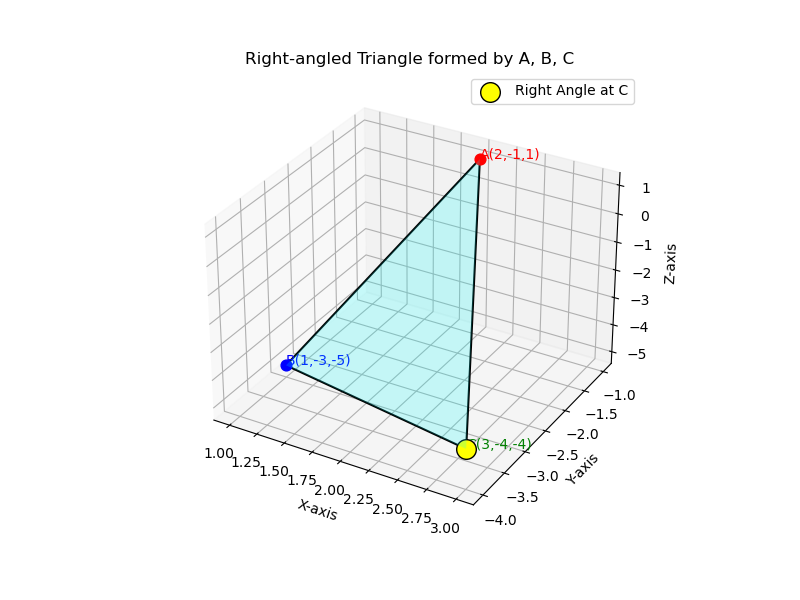
\includegraphics[width=\columnwidth, height=0.8\textheight, keepaspectratio]{Figs/Fig1.png}     
\end{frame}



\end{document}